% This is "sig-alternate.tex" V2.1 April 2013
% This file should be compiled with V2.5 of "sig-alternate.cls" May 2012
%

\documentclass[english,conference]{IEEEtran}

%\usepackage{cite} % recommended by IEEEtran template

\usepackage{babel}
\usepackage{csquotes}
\MakeOuterQuote{"}

%\usepackage[backend=biber,style=numeric-comp]{biblatex}
%\bibliography{references}
%\renewcommand{\bibliography}[1]{\printbibliography}

\usepackage{lmodern}
\usepackage{MnSymbol}

\usepackage[svgnames]{xcolor}
%\usepackage{todonotes}
%\presetkeys{todonotes}{inline}{}
\usepackage[subject={TODO}]{pdfcomment}
\newcommand{\todo}[2][]{\pdfmargincomment[author={#1}]{#2}}

%\usepackage{makecell}
\usepackage{ctable}
\newcolumntype{R}{>{\raggedleft \arraybackslash}X}


\usepackage{listings}

\newcommand{\lineref}[2]{\hyperref[#1]{line~\ref*{#1:#2}}}
\newcommand{\linerefn}[2]{\hyperref[#1]{line~#2}}
\newcommand{\linesrefn}[2]{\hyperref[#1]{lines~#2}}
\usepackage{accsupp}
\newcommand\emptyaccsupp[1]{\BeginAccSupp{ActualText={}}#1\EndAccSupp{}}

\usepackage{hyperref}
\usepackage[all]{hypcap}
\PassOptionsToPackage{nameinlink,noabbrev}{cleveref}
\usepackage{cleveref}


\lstset{captionpos=b}
\lstset{basicstyle=\small\ttfamily}
\lstset{showstringspaces=false, columns=flexible, keepspaces=true}
\lstset{tabsize=2, gobble=2}
\lstset{upquote=true}
%% Linebreaks
%\lstset{prebreak=\raisebox{0ex}[0ex][0ex]
%        {\ensuremath{\rhookswarrow}}}
\lstset{postbreak=\raisebox{0ex}[0ex][0ex]{\ensuremath{\rcurvearrowse\space}}}
\lstset{breaklines=true, breakatwhitespace=true}
%% Line Numbers
\newcommand{\lstnumberstyle}[1]{\tiny\emptyaccsupp{#1}}
\lstset{numbers=left, numberstyle=\lstnumberstyle, numbersep=5pt,
		numberfirstline=true, firstnumber=1, stepnumber=5}
\lstset{escapeinside={(*@}{@*)}}

\lstdefinestyle{BWStyle}{
	keywordstyle=\bfseries,
	stringstyle=\color{DimGray},
	commentstyle=\textsl,
}
\lstset{style=BWStyle}

\lstdefinelanguage{algorithm}{
	keywords={function, for, do, if, then, else, return, in_, is_a, or, and},
	morecomment=[l]{'},
	morecomment=[s]{/*}{*/},
	morestring=[b]",  
	sensitive=true,
}
\lstdefinelanguage{HanaSQL}[]{SQL}{
	morekeywords={replace,string,if,is,daysbetween,secondsbetween,weekday,adddays,addseconds,double, procedure,begin,declare,inout,call,return,returns},
	moredelim=**[is][\slshape]{^}{^},
	moredelim=**[is][\bfseries]{§}{§},
}
\lstdefinelanguage{Inline}{
	moredelim=**[is][\slshape]{^}{^},
	moredelim=**[is][\bfseries]{§}{§},
}

\lstset{language=HanaSQL}
\lstMakeShortInline[basicstyle=\ttfamily,language={Inline},breaklines=true]°

%Macros
\newcommand{\tool}{TAR\-DISP}
\newcommand{\SQLextension}{Back-in-time SQL}


\begin{document}

\title{Bringing Back-in-Time Debugging\\ down to the Database}
%\subtitle{(\tool is a placeholder for the actual name)}

\author{\IEEEauthorblockN{Arian Treffer}
\IEEEauthorblockA{Hasso-Plattner-Institut\\
Potsdam, Germany\\
arian.treffer@hpi.de}
\and
\IEEEauthorblockN{Michael Perscheid}
\IEEEauthorblockA{SAP Innovation Center\\
Potsdam, Germany\\
michael.perscheid@sap.com}
\and
\IEEEauthorblockN{Matthias Uflacker}
\IEEEauthorblockA{Hasso-Plattner-Institut\\
Potsdam, Germany\\
matthias.uflacker@hpi.de}}


%\numberofauthors{3} 
%\author{
%% 1st. author
%\alignauthor
%Arian Treffer\\
       %\affaddr{Hasso-Plattner-Institut}\\
       %\affaddr{Potsdam, Germany}\\
       %\affaddr{arian.treffer@hpi.de}
%% 2nd. author
%\alignauthor
%Michael Perscheid\\
       %\affaddr{SAP Innovation Center}\\
       %\affaddr{Potsdam, Germany}\\
       %\affaddr{michael.perscheid@sap.com}
%% 3rd. author
%\alignauthor 
%Matthias Uflacker\\
       %\affaddr{Hasso-Plattner-Institut}\\
       %\affaddr{Potsdam, Germany}\\
       %\affaddr{matthias.uflacker@hpi.de}
%%\and  % use '\and' if you need 'another row' of author names
%}

%\date{30 July 1999}

\maketitle
\begin{abstract}
Back-in-time debuggers allow developers to explore what happened before a failure and so support them in finding failure causes more efficiently. 
However, if failure causes leave a specific application layer, it is difficult to further follow infections down to the real defect.
Especially at the database-level, developers have no such debugging tools to understand unexpected behavior comprehensively.

In this paper, we present an approach for bringing back-in-time debugging down to SQL and stored procedures of the SAP HANA in-memory database.
Our \tool\ debugger allows developers to step queries backwards and inspecting the database at previous and arbitrary points in time.
With the help of a SQL extension, we can express queries covering a period of execution time within a debugging session and handle large amounts of data with low overhead on performance and memory.
The entire approach has been evaluated within a development project at SAP and shows promising results with respect to the gathered developer feedback.
\end{abstract}

%\keywords{Back-in-time debugging, in-memory database, SAP HANA}

%%%---------------------------------------------------------------------------------------------------------------------------------------------------------------------------------
%%%---------------------------------------------------------------------------------------------------------------------------------------------------------------------------------
%%%---------------------------------------------------------------------------------------------------------------------------------------------------------------------------------

\section{Introduction}

%Context: Debugging and Back-in-Time
Finding defects in code is a frequent task for every programmer and is often difficult even with a deep understanding of the system.
To localize failure causes, they examine involved program entities and distinguish relevant from irrelevant behavior and clean from infected state. 
However, common symbolic debuggers do not support identification of such infection chains very well because they only provide access to the last point of execution without access to the program history.
Back-in-time also known as omniscient debuggers simplify the debugging process by making it easier to follow cause-effect chains from the observable failure back to the causing defect~\cite{lewis_debugging_2003}.
These tools provide full access to past events so that developers can directly experiment with the entire infection chain. 

%Problem: Back-in-time debugger missing for database-level
Even though back-in-time debuggers exist for many object-oriented programming languages~\cite{feldman_igor:_1988,hofer_design_2006,lewis_debugging_2003}, there are none to the best of our knowledge that run on databases and support SQL or SQLScript\footnote{SQLScript is a proprietary SQL extension for stored procedures in SAP HANA~\cite{sqlScript}.}.
This is mainly because of two reasons. 
First, back-in-time debuggers typically create a significant overhead on performance and memory consumption~\cite{lewis_debugging_2003,lienhard_practical_2008,pothier_scalable_2007}.
It seems unfeasible to use a back-in-time debugger on top of a database script that processes billions of records.
Second, current back-in-time debugging concepts cannot handle side-effects outside their system that usually happen in writing operations during INSERT and UPDATE statements. 

%Significance: Especially, in business software much development is based on database scripts. 
Due to high performance requirements of handling big data in business applications, SAP has not only a strong demand to move code closer to data~\cite{plattner2015memory} but also the need to improve development tools at the database-level. 
As existing tools mostly work on the application level, are limited to specific points in time, or work only on a query plan, developers are often left alone when it comes to debug and understand the results of their SQL and SQLScripts.
We argue that a back-in-time debugger at the bottom of the technology stack is able to close this gap and would support developers in developing and maintaining their queries more efficiently. 

%Solution
In this paper, we bring the concept of back-in-time debugging to the database and present \emph{\tool} as an implementation of our approach.
The contributions of this paper are as follows:
\begin{itemize}
	\item \emph{\tool} is a back-in-time debugger for stored procedures which can be installed in the SAP HANA in-memory database and programming platform.
		Using \tool, developers can move freely through the execution time of a stored procedure and inspect control flow, variables, and intermediate results.
	
	\item \emph{\SQLextension} is an extension to SQL allowing to submit arbitrary queries against previous states of the database 
		and to compare multiple points in time with one query.
		\tool\ provides a console for developers to submit \SQLextension\ queries which use variables or points in time from the current debug session.

	\item \emph{Very low overhead} when recording run-time data and the efficient querying of past database states allow developers to use \tool\ as the default tool for debugging database scripts even on larger data sets.
	
\end{itemize}

We evaluated \tool\ with the help our SAP colleagues who worked on a project called \emph{Point of Sales Explorer}~\cite{plattner2015memory} which makes heavy use of SQLScript. 
The interviews indicated that bugs in stored procedures can be investigated more efficiently with \tool\ than with existing other database development tools.

The remainder of this paper is structured as follows:
\Cref{sec:relatedWork} describes related work. 
\Cref{sec:prototype} presents our approach and its prototypical implementation of back-in-time debugging in the database.
\Cref{sec:ttqueries} discusses querying past database states and introduces and extension to SQL.
\Cref{sec:evaluation} evaluates our approach before \cref{sec:conclusion} discusses future work and concludes the paper.

%%%---------------------------------------------------------------------------------------------------------------------------------------------------------------------------------
%%%---------------------------------------------------------------------------------------------------------------------------------------------------------------------------------
%%%---------------------------------------------------------------------------------------------------------------------------------------------------------------------------------

\section{Related Work}
\label{sec:relatedWork}

The first debugger that could reverse execution was EXDAMS for FORTRAN in the late 1960s~\cite{balzer_exdams:_1969}, which stored old program state on tape.
Later, other reversible debuggers used memory snapshots~\cite{feldman_igor:_1988} or reversible execution~\cite{lieberman1997zstep} to allow stepping backwards through time.

The \emph{omniscient debugger}~(ODB)~\cite{lewis_debugging_2003} was the first debugger to keep the entire program history in memory.
This allows fast jumping between arbitrary points in time and querying the execution history, but creates a large overhead on runtime and memory consumption.
The trace-oriented  debugger (TOD)~\cite{pothier_scalable_2007} uses a specialized distributed database to better handle large amounts of trace data.
Object  flow  analysis~\cite{lienhard_practical_2008} reduces the required amount of memory by using the VM's garbage collector to discard objects and events that are no longer reachable.

%%%---------------------------------------------------------------------------------------------------------------------------------------------------------------------------------
%%%---------------------------------------------------------------------------------------------------------------------------------------------------------------------------------
%%%---------------------------------------------------------------------------------------------------------------------------------------------------------------------------------


\section{Back-in-time Debugging for\\ Stored Procedures}
\label{sec:prototype}

% why post mortem
\todo{If we need to shorten later on, I would start here in the problem description.}
With a regular debugger, developers have only one way to go back in time, which is to restart the execution.
Tools can be used to automate this approach\todo{cite checkpoint debugger?} and some modern debuggers even allow to restart execution at the method level\todo{http://help.eclipse.org/neon/index.jsp?topic=\%2Forg.eclipse.jdt.doc.user\%2Freference\%2Fviews\%2Fdebug\%2Fref-droptoframe.htm}.
However, this approach fails if the code has side effects, as it can no longer be guaranteed to execute in the same way.
Furthermore, if the execution is too slow, developers will spend much time waiting for re-execution, which discourages the use of backwards stepping.

A different way to examine a program's behavior over time is to record a trace of the program's actions.
After the program terminated, the trace can be examined in a post-mortem analysis.
This works well for special purpose tools that only analyze a specific aspect of a program, such as profilers.
A post-mortem debugger, on the other hand, has to record virtually everything to be able to replay the program execution.
While this approach allows developers the most freedom when stepping through the execution, it creates a large overhead on performance and memory.
Debugger implementations using this approach exist for different programming languages.
%
Both approaches can also be mixed to create a tradeoff between performance and overhead\todo{cite}.

% post-mortem has been solved before, why is it harder in the database
When debugging programs that run on a database, a back-in-time debugger faces two additional problems:
First, the program's behavior strongly depends on external state.
With live debugging, this sometimes can be mitigated by resetting the database before restarting the program, but a post-mortem analysis can not easily examine intermediate states when they have been changed.
Second, much of the data processing happens outside of the program's scope.
Sometimes, state that has impact on a query's result even remains entirely in the database and is practically invisible to analysis tools.
The only way to examine such state is through specific database queries before it is changed.

Stored procedures add the additional challenge that results of a query can be used in subsequent database statements without having been fetched into the program.
This increases the amount of "invisible" state, sometimes only for a few instructions, other times for the entire length of the program.
Furthermore, as trace data usually exceeds program data by orders of magnitude, we expect that tracing the processing of every tuple in a large database is not feasible.

With \tool, we focuses on stored procedures because they are executed close to the data and, thus, more efficient in handling large data sets.
This does not limit the general validity of our results, as a stored procedures debugger faces all of the challenges described above.

\subsection{Replaying a Stored Procedure}

While using a database to manage application state creates several problems for debugging tools, it also opens up new possibilities to simplify or improve the debugger.

First, the database persists state beyond the program execution.
Even post-mortem, the state can be directly accessed by the debugger.

Second, all instructions handling large data sets (i.e., SQL statements), are declarative.
This means they can be analyzed without knowing how they are physically executed and results are reproducible as long as the underlying data does not change.
%Thus, SQL queries don't have to be traced at all, although for some purposes it will be helpful to record some meta information, such as the execution time or the number of results.
Thus, neither do we need to trace the internals of a query's execution, nor do we need to persist the query result.
\todo{MP: This is not clear to me, yet.}

Third, the database can be used to efficiently manage old state.
In-memory databases with insert-only storage automatically retain old data~\cite{Plattner2009Acd}.
With insert-only, older versions of the database can be easily reproduced.
For other databases, insert-only can be achieved by adding validity columns.
For many business applications, such columns already exist where no data may be deleted for legal reasons.

In conclusion, all that is needed to reproduce the execution of a stored procedure is a sequence of execution steps.
Each step represents an instruction that has side effects on the database or assigns a value or result set to a variable.
As there is, conceptually, no concurrency in a stored procedure, we can use sequential numbering to track the order of steps.

If applicable, a step has a target name, such as the name of a variable or stored procedure, and a string representation of the value, which can be shown to the user in the debug view.
If the step involves a database statement, we only need a timestamp to be able to reproduce the query.
Moreover, we also record the number of rows in the result set and the execution time, as well as any atomic argument values, as this information is likely to be relevant for developers.

%We never trace any details of the query execution but only record the name of a view than can be used to later reproduce the query result.
%The view was specifically generated by the debugger, as will be explained in the next subsection.

%\subsection{Reproducing Query Results}

With the recorded trace data, the debugger has enough information available to replay the execution and to re-execute any query.
%
%However, the query will only yield the same results as long as the underlying data has not changed.
%
%In general, one can expect that debugging will take place on a development machine where no other data manipulation occurs.
%However, in cases where this assumption doesn't hold, the debugger might end up showing wrong or misleading data the developer.
%Furthermore, the debugged stored procedure itself may change the data, which will cause a query to return different results at different points in time.
%
%We ensure consistency over time by following the insert-only approach of our in-memory database.
%If we require for all tables that data can never be changed or deleted and annotate all tuples with timestamps of when they have been created and invalidated, we can reconstruct the state of the database of any point in time.
%Adding timestamp filters to select queries does not cause a significant slowdown.
%Our prototype was built using this approach.
%\todo{HANA hat seit neustem "History tables" die das direkt können, wir benutzen aber explizite timestamps weil das momentan noch praktischer ist }


\subsection{Prototype and Tracing Code Generation}

We developed \tool\ as a prototype implementation of our approach.
Our back-in-time debugger runs in the SAP HANA XS-Engine, a framework for web-applications that is part of the SAP HANA platform.
The user interface is written in HTML5 and JavaScript and queries debugging data via HTTP from the back-end, written in server-side JavaScript.
Traces are stored directly in the database.
Packaged as a XS Application, \tool\ can be directly deployed in a SAP HANA installation.

%With a debugger fully integrated in its database, we would expect the stored procedure execution engine to trace the execution steps.
%However, for our prototype this level of integration was out of scope.\todo{Don't start this way but rather put it into limitation discussion or next steps in summary and than call it producterization}

To be able to trace an execution, we developed a SQLScript pre-processor that parses a stored procedure and adds °INSERT° statements around every instruction to collect the required trace data.
To obtain a trace, the debugger then once has to run the traced code instead of the original procedure.

In addition to the tracing code, the pre-processor also generates SQL functions and views that will be used to obtain variable values at given points in time.
For atomic variables, it is simply a search for its most recent step.

For variables containing result tables, a separate view is generated for each query that assigns to that variable.
Each view contains the original code of its query.
Arguments to the query are initialized using their respective views.
On top of that, a master view is generated that chooses the appropriate query view by looking up the requested step in the recorded trace.
%\todo{AT: How much detail?}

\begin{figure}
	\centering
		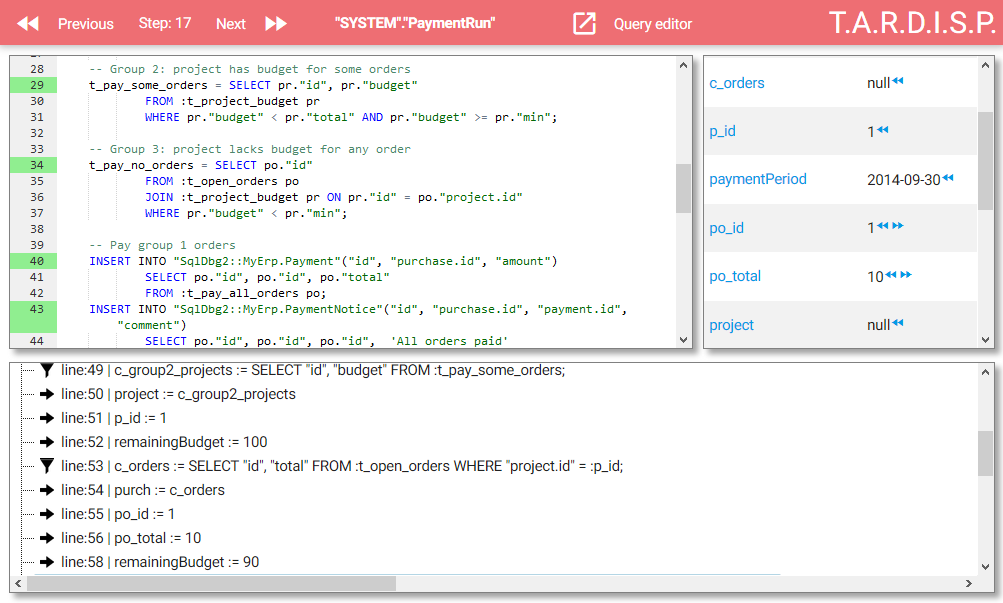
\includegraphics[width=\linewidth]{odb.png}
	\caption{User interface of the \tool\ debugger.}
	\label{fig:odb}
\end{figure}

The user interface looks like a typical debugger and is is shown in \cref{fig:odb}.
The top-left part of the screen shows the code.
Above, a toolbar contains buttons allowing developers to step forwards and backwards.
Between the step buttons, the current step number is shown.
Below, \tool\ shows a tree of all execution steps instead of a stack trace.

Next to the code, current variable values are shown.
Arrow buttons allow to jump to the previous or next assignment of the variable.
For variables containing a query result, the size of the result is shown.
Clicking the variable opens a query window that shows the variable's content and allows the developer to submit time-travel queries, which will be explained in the next section.

%%%---------------------------------------------------------------------------------------------------------------------------------------------------------------------------------
%%%---------------------------------------------------------------------------------------------------------------------------------------------------------------------------------
%%%---------------------------------------------------------------------------------------------------------------------------------------------------------------------------------

\newcommand{\red}[1]{\textcolor{DarkRed}{#1}}
\newcommand{\gr}[1]{\textcolor{Green}{#1}}
\newcommand{\timediffresult}{
\ctable[star,caption={Result of a time-diff query, with multiple values in some columns. Red indicates a different value at the \emph{before} step, green indicates a different value at the \emph{after} step.},label=tab:diffresult,doinside={}]
				{rlrrrlr}{}{
	pr.id & pr.name 	& pr.budget  & total & po2.id & po2.status & po2.total \ML
	
				&					  & \red{1200} & \red{1500} &	  & \red{open} &					\NN
	1			& Project 1 & 200			 	 & 500 			  & 1 & paid 			 & 1000			\NN
				&						& \gr{-300}  & \gr{0}		  &	  &						 &					\ML

				&					  & \red{1200} & \red{1500} &	  & 					 &					\NN
	1			& Project 1 & 200				 & 500 			  & 2 & open 			 & 500			\NN
				&						& \gr{-300}  & \gr{0}		  &	  & \gr{paid}	 &					\ML
}
}

\timediffresult

\section{\SQLextension}
\label{sec:ttqueries}

In our setup, the debugger has to recreate intermediate results of a stored procedure.
We generalized this feature to enable developers to submit arbitrary queries against the database of any previous point in time.
Furthermore, we allow developers to compare query results from different points in time and even query for changes in the data.
We defined \SQLextension, a super-set of SQL that allows developers to refer to points in execution time by introducing a new keyword and a new operator.

\subsection{A SQL Clause to Query Points in Time}

As an example, we consider a stored procedure that triggers the payment of purchase orders.
Users reported a bug: projects sometimes exceed their budget, which is not supposed to happen.

Developers might start debugging this issue and the related stored procedure with \tool.
However, they soon realize that the number of projects is too large to continue stepping manually.
Instead, they open \tool's SQL console and submit the query shown in \cref{lst:ttravel} to look into the °select_projects° variable, which contains ids, names, and budgets of all projects to be processed.
To better understand the data, they also sum up the total amount of all open purchase orders for each project.

%\Cref{lst:ttravel} shows the query to fetch all selected projects together with the total amount of open orders\todo{The previous paragraph already explains the code - reference to listing needs to be earlier.}.
%We will use it as an example to show how \tool\ handles time-travel queries.

%\begin{figure} % IEEE says put code in figures
%\begin{lstlisting}
\begin{lstlisting}[language=HanaSQL,float,caption={Example for a time-travel query: select the current total of open orders for previously selected projects},label=lst:ttravel]
  SELECT pr.id, pr.name, pr.budget, SUM(po.total)
  FROM :selected_projects pr
	JOIN PurchaseOrders po ON po.project_id = pr.id
	WHERE po.status = 'open'
	GROUP BY pr.id, pr.name, pr.budget
	^§AT STEP§ 1623^
\end{lstlisting}
%\caption{Example for a time-travel query: select the current total of open orders for previously selected projects}
%\label{lst:ttravel}
%\end{figure}

The last line of \cref{lst:ttravel} contains the °^AT STEP^° clause, our extension to SQL that allows developers to explicitly query a specific point in time.
When opening the SQL console, \tool\ automatically provides an °AT STEP° clause with the number of the current debug step, °^1623^° in this case.
Developers can obtain numbers for other steps from the stepping toolbar or the execution tree. 

When submitted, \tool\ applies two transformations to the query before it is passed to the database.
First, all variables are replaced with their corresponding functions or views that were generated during the pre-processing of the stored procedure.
Each function or view receives the specified step number as an argument to be able to produce the correct value or table.
Second, time-stamp filters on the validity columns are added for all tables that are referenced in the query. 
Because of SAP HANA's insert-only approach, this lets all tables appear exactly as they originally were at the specified point in time.
\todo{Refere again to the insert-only feature of SAP HANA that allows this approach}

%In our example,
%\begin{lstlisting}[language={Inline},basicstyle=\ttfamily,numbers=none]
  %po.createdOn < ^1623^ AND (po.validTo IS NULL OR po.validTo > ^1623^)
%\end{lstlisting}
%would be added to the where-clause.

Now, the query can be submitted to the database and the result is subsequently presented to the user.

When developers omit the step number, it is taken from the context of the debug session.
This way, developers can step through the execution and observe how the query result changes over time.

\subsection{Time-diff Queries}

Furthermore, \SQLextension\ provides an easier way to find the origin of changes in the data.
To get a better overview about what happened in a segment of code, developers might want to query multiple points in time at once and see the difference in the query result.
In our example, developers are looking for purchase orders that cause projects to exceed their budget.
Using \tool, they identified three important points in time, which we will call \emph{before}, \emph{now}, and \emph{after}.
\emph{Before} is the step where the stored procedure started processing purchase orders, \emph{now} is the current step, and \emph{after} is the final step of the procedure.

In \cref{lst:tdiff}, the query from above was extended to select individual purchase orders for each project.
In line 10, the at-step clause now specifies all three points in time.
This allows developers to query for changes in the data.

Because the steps are named, they can now be used in the query as time qualifiers.
\SQLextension\ introduces the exclamation mark operator that binds an identifier to a step.
In line 6, it is used to limit the search to projects that will exceed their budget before the stored procedure ends;
in line 7, it is used to filter for purchase orders whose status was or will be changed.

%\begin{figure} % IEEE says put code in figures
%\begin{lstlisting}
\begin{lstlisting}[language=HanaSQL,float=b,caption={Example of a time-diff query: "Select all projects that will go over budget and their respective purchase orders"},label=lst:tdiff]
	SELECT pr.id, pr.name, pr.budget, SUM(po.total), po2.id, po2.status, po2.total
	FROM :selectedProjects pr
	JOIN PurchaseOrders po ON po.project_id = pr.id
	JOIN PurchaseOrders po2 ON po2.project_id = pr.id
	WHERE po.status = 'open'
		AND ^now!^pr.budget > 0 AND ^after!^pr.budget < 0
		AND ^before!^po2.status != ^after!^po2.status
	GROUP BY pr.id, pr.name, pr.budget, 
	         po2.id, po2.status, po2.total
	^§AT STEP§ before=817, now=1623, after=2043^
\end{lstlisting}
%\caption{Example of a time-diff query: "Select all projects that will go over budget and their respective purchase orders"}
%\label{lst:tdiff}
%\end{figure}

\Cref{tab:diffresult} shows a possible result for this query, with one project that goes over budget and two associated purchases.
The values for budget and total of outstanding payments are shown for each of the three steps.
Of the two purchase orders, the first was already marked as "paid" before the current step, the other is about to be paid.

Analyzing this data, it becomes clear that the payment of the second order is what causes the project budget to become negative.
\todo{What is the budget limit, difficult to see for reader... needs a bit more explanation}
Developers can now click on the green "paid" value to jump exactly to the point in time where this order is updated, knowing that at this point they are very likely to be close to the bug they are looking for.

To produce this result, the query has to be executed three times, once for each point in time, without the time-specific where-conditions.
The partial results are outer-joined on the primary key attributes, then the time-specific filter conditions are applied.
\tool\ rewrites the query to fit everything into a single select statement, which allows the database to compute the entire result in one request.

The final query selects all values from each sub-query.
In the user interface, changes in the values are highlighted in as shown in \cref{tab:diffresult}.
If a value changed since the \emph{before} step, the old value is shown red; if a value will change until the the \emph{after} step, the new value is shown green.
\todo{what means red and what green? Also add explanation of colors to caption of table}
When possible, the tuple creation timestamps are used to allow developers to jump exactly to the point in time where the change occurred.

%Then, to prepare the diffing of the results, they are outer-joined on the primary keys and the time-specific filters are applied.
%For performance reasons, all of this happens inside a single SQL query, as shown in \cref{lst:tdifffinal}.
%The execution of the sub-queries is indicated in \linerefn{lst:tdifffinal}{6, 7, and 10}, the time-specific filters can be found in the Where-condition of \linerefn{lst:tdifffinal}{15 and 16}.

%
%In the UI\todo{Instead of many code listing show the UI (this could also include the code)}, the before and after values are only shown if they differ from the now value.
%Clicking on value allows the developer to jump to the °UPDATE° or °INSERT° statement that caused the change.

%%%---------------------------------------------------------------------------------------------------------------------------------------------------------------------------------
%%%---------------------------------------------------------------------------------------------------------------------------------------------------------------------------------
%%%---------------------------------------------------------------------------------------------------------------------------------------------------------------------------------

\section{Evaluation}
\label{sec:evaluation}

We evaluated our \tool\,debugger on a real-world SAP project that has been developed in co-innovation with one of the largest European retail companies. 
This project is called \emph{Point of Sales Explorer}~\cite{plattner2015memory} and allows category managers to see a collection of the most important key performance indicators (KPIs) for several thousands of products in a unified dashboard.
Based on more than 2 billion records of point of sales data, this application aggregates on the fly the requested KPIs with the help of SAP HANA and allows users to further refine them by stores, vendors, or products as they like. 
In order to implement flexible requests such as returning the revenue and margin per week of current and last year, this application makes heavy use of SQLScript. 
For that reason, it is a proper candidate to measure performance and interview its developers with respect to our \tool\ tool. 

\subsection{Performance Measurements}

Each value is the average of 10 measurements.

To evaluate the performance of our approach, we deployed \tool\ on a copy of the Point of Sales system.

We selected two stored procedures from the Point of Sales Explorer and compared the runtime with and without tracing.
%To measure the impact of database size, 
We ran each procedure with different arguments that would lead to intermediate results of different sizes.
The results are shown in \cref{tab:measure1}.
Each value is the average of 10 measurements.
We found the overhead of tracing to be consistently between 6 and 7 percent.

\ctable[caption={Average execution time for running a stored procedure without and with tracing and for reproducing its result.},label=tab:measure1,doinside={},width=\linewidth]
				{llRRR}{}{
				&		& Normal run& Run with tracing  & Reproducing the result \ML
	
			&	(a) &	1.27 s		& 1.35 s		& 1.21 s		\NN
Proc.1& (b)	&	1.61 s		& 1.74 s		& 1.54 s		\NN
			&	(c) &	1.73 s		& 1.85 s		& 1.60 s		\ML

			&	(a) &	1.24 s		& 1.32 s		& 1.19 s		\NN
Proc.2& (b)	&	1.61 s		& 1.72 s		& 1.55 s		\NN
			&	(c) &	1.69 s		& 1.80 s		& 1.63 s		\ML
}

We also measured the time it takes to reproduce result of each stored procedure.
This provides us with an upper bound for how long \tool\ would need to compute the value of any variable because in our examples all variables are needed to compute the final result.
The measurements in \cref{tab:measure1} show that reproducing the result is slightly faster than executing the stored procedure.
This was expected because for variables containing atomic values the value could be taken directly from the trace.
Only for variables containing table results, database queries had to be executed again.

Finally, we selected two queries from the stored procedures as examples for queries a developer might submit through the debugger's SQL console and measured their execution time both as a regular query and as a time-diff query.
Because the Point of Sales Explorer only computes KPIs and does not change the data, we let the time-diff query compare different time-spans of point of sale data\todo{is this disclaimer needed?}.
Again, we used different filter arguments to produce different result sizes.
As \cref{tab:measure2} shows, in each case the runtime overhead of time-diff queries is around 25 percent.

\ctable[caption={Average execution times for queries executed normally or as time-diff query.},label=tab:measure2,doinside={},width=\linewidth]
				{llRR}{}{
				&		& Regular query& Time-diff query \ML
	
			 &	(a) &	1.21 s		& 1.51 s	\NN
Query 1& (b)	&	1.74 s		& 2.12 s	\NN
			 &	(c) &	1.79 s		& 2.23 s	\ML

			 &	(a) &	61 ms		&  75 ms	\NN
Query 2& (b)	&	81 ms		& 100 ms	\NN
			 &	(c) &	88 ms		& 109 ms	\ML
}

\subsection{Interviews}

Besides measuring performance, we also demonstrated our back-in-time debugger to two backend developers of the Point of Sales Explorer. 
These persons have written most of the SQLScript and so know all the challenges when developing close to the database. 
Both had the chance to apply \tool\ in their daily work while we provided tool support and observed them in the background. 
Finally, we've conducted an in-depth interview in order to receive feedback and further improve our tool.

We found out that the main reason for writing SQLScript is to positively influence the optimizer of SAP HANA in order to speed up the overall user request.
This worked very well as long as the newly written code was bug-free. 
However, if something went wrong at the database-level, the existing tool support was not sufficient. 
They often had to guess why a specific sub query was not as expected. 
For that reason, they liked our back-in-time debugger and we received a lot of positive feedback.
For example, \tool\ could not only show formerly hidden results but also helped them to understand and follow back the reasons behind a failure cause. 
The greatest improvement was reported for debugging stored procedures that take a table of data as an argument.
Composing such an argument with specific data using the existing tools is cumbersome and has to be redone every time the debug session has to be restarted.
Using \tool, it has to be done only once.
Besides that, both developers also revealed several small bugs in our debugger and wished for some new features such as the ability to define temporary tables for testing code and queries.
With this feedback, we see a strong need for better debugging support at the database-level and are eager to further improve our approach.

%\subsection{Threats to Validity}

\subsection{Limitations}

Our implementation of \SQLextension currently has two limitations.

First, time-diff queries can only be executed on tables that have clearly defined primary keys because key attributes are required to track a tuple's versions over time.
For a query like "Sum budgets per project category", it has to be clear that categories are the entities that keep their identity over time.
Here, an additional syntax extension could be used to convey this kind of information.

Second, it is currently not possible to use time qualifiers on identifiers outside of the where clause.
We can imagine that there may be a need to use time qualifiers in other SQL clauses, such as the select or order-by clause.
In other use cases, developers might want to attach a time qualifier directly to a table.

%%%---------------------------------------------------------------------------------------------------------------------------------------------------------------------------------
%%%---------------------------------------------------------------------------------------------------------------------------------------------------------------------------------
%%%---------------------------------------------------------------------------------------------------------------------------------------------------------------------------------

\section{Conclusion}
\label{sec:conclusion}

We presented an approach for bringing back-in-time debugging down to SQL and stored procedures, and the \tool\ debugger, an implementation of our approach that runs on the SAP HANA in-memory database.
With \tool, developers can step forwards and backwards through the execution of a stored procedure.
We introduced \SQLextension, a super-set of SQL, that allows developers to query the database from any point in the execution, compare the data of multiple points in time with one query, and even query for changes in the data.

Our evaluation has shown that the runtime overhead caused by execution tracing is small enough to let \tool\ be the default choice for debugging stored procedures.
Interviews with developers have confirmed the usefulness of back-in-time debugging for finding bugs in database programs.

Future work will move in two directions.
First, we shall bring more advanced debugging techniques that use a combination of trace data and code analysis to help identify bugs, such as dynamic slicing~\cite{agrawal_dynamic_1990} or why-questions~\cite{ko_debugging_2008}, down to the database.
Second, while developers now have the tools to efficiently debug each layer of a complex application, the tool support to track bugs across layers and system boundaries is still lacking.
We want to develop a back-in-time debugger that will allow developers to debug seamlessly across application layers.


%
% The following two commands are all you need in the
% initial runs of your .tex file to
% produce the bibliography for the citations in your paper.
\bibliographystyle{abbrv}
\bibliography{sigproc}  % sigproc.bib is the name of the Bibliography in this case

\end{document}